% GHOST system model with the real intermediate tensors of one request
% (ResNet-20, split after block 3, rho = 10, CIFAR-10 test image 1398; layer blocks.0.conv1 shown),
% produced by ghost2/fig_tensors.py. Drawn at IEEE \textwidth (7.16in).
\documentclass[tikz,border=1pt,10pt]{standalone}
\usepackage[T1]{fontenc}
\usepackage{mathptmx}
\usepackage{courier}
\usepackage{graphicx}
\usetikzlibrary{arrows.meta,calc}
\definecolor{ink}{HTML}{1A1A1A}
\definecolor{dark}{HTML}{263238}
\definecolor{teeC}{HTML}{2E7D32}\definecolor{teeF}{HTML}{EDF6EE}
\definecolor{reeC}{HTML}{C62828}\definecolor{reeF}{HTML}{FCEDED}
\definecolor{clC}{HTML}{1565C0}\definecolor{clF}{HTML}{EAF2FB}
\definecolor{setC}{HTML}{6A1B9A}\definecolor{setF}{HTML}{F4EEF8}
\definecolor{devC}{HTML}{37474F}
\definecolor{acc}{HTML}{E65100}
\definecolor{bar}{HTML}{4A6FA5}
\def\TokHex{e1817c66}
\def\CtHex{d06c51cc}
\def\PredClass{Horse}
\def\ProbList{0.056,0.000,0.013,0.041,0.001,0.066,0.000,0.813,0.008,0.002}
\def\WRows{16}\def\WtRows{20}

\graphicspath{{arch_assets/}}
\tikzset{
  >={Stealth[length=2mm,width=1.6mm]},
  font=\footnotesize, every node/.style={text=ink},
  zone/.style={draw=#1,line width=1pt,rounded corners=2.5pt},
  tab/.style={fill=#1,text=white,font=\small\bfseries,inner xsep=3pt,inner ysep=2pt,rounded corners=1.5pt},
  vtab/.style={fill=#1,text=white,font=\footnotesize\bfseries,rotate=90,inner xsep=3pt,inner ysep=2pt},
  ttl/.style={align=center,inner sep=0.6pt,font=\footnotesize},
  f/.style={->,draw=dark,line width=0.85pt},
  fo/.style={->,draw=setC,line width=0.85pt,dash pattern=on 3pt off 1.8pt},
  bridge/.style={preaction={draw=white,line width=3.4pt,-}},
  n/.style={circle,draw=dark,line width=0.7pt,fill=white,text=dark,font=\footnotesize\bfseries,inner sep=0pt,minimum size=4mm},
  lab/.style={font=\footnotesize,inner sep=1pt},
}
% stack of four channel maps: front tile #4, offset 0.1cm, centred at (#1,#2)
\newcommand{\fstack}[4][0.82]{%
  \pgfmathsetmacro{\hw}{(#1+0.3)/2}
  \foreach \k in {3,2,1,0}{%
    \node[inner sep=0pt,anchor=south west,draw=ink,line width=0.3pt]
      at ({#2-\hw+\k*0.1},{#3-\hw+\k*0.1}) {\includegraphics[width=#1cm]{#4\k}};}}
\newcommand{\tile}[4]{\node[inner sep=0pt,draw=ink,line width=0.4pt] at (#1,#2) {\includegraphics[width=#4]{#3}};}
\newcommand{\inset}[4][0.42]{\node[inner sep=0pt] at (#2,#3) {\includegraphics[width=#1cm]{#4}};
  \draw[white,line width=0.9pt] ($(#2,#3)+(-#1/2,-#1/2)$) rectangle ++(#1,#1);
  \draw[ink,line width=0.4pt] ($(#2,#3)+(-#1/2,-#1/2)$) rectangle ++(#1,#1);}
\newcommand{\padlock}[3][1]{%
  \begin{scope}[shift={(#2,#3)},scale=#1]
   \draw[dark,line width=1.2pt] (-0.1,0.09) -- (-0.1,0.18) arc (180:0:0.1) -- (0.1,0.09);
   \fill[dark,rounded corners=1pt] (-0.17,-0.15) rectangle (0.17,0.11);
   \fill[white] (0,-0.02) circle (0.04);
  \end{scope}}
\newcommand{\shield}[4][1]{% x y colour
  \begin{scope}[shift={(#2,#3)},scale=#1]
  \fill[#4] (0,0.42) .. controls (0.2,0.34) .. (0.32,0.34) -- (0.32,0.04) .. controls (0.32,-0.23) .. (0,-0.38)
              .. controls (-0.32,-0.23) .. (-0.32,0.04) -- (-0.32,0.34) .. controls (-0.2,0.34) .. cycle;
  \draw[white,line width=1.4pt,line cap=round,line join=round] (-0.15,0.0) -- (-0.03,-0.12) -- (0.17,0.15);
  \end{scope}}
\newcommand{\chip}[3][1]{%
  \begin{scope}[shift={(#2,#3)},scale=#1]
  \foreach \j in {-0.2,-0.07,0.07,0.2}{
    \draw[dark,line width=0.6pt] (\j,0.3) -- (\j,0.4); \draw[dark,line width=0.6pt] (\j,-0.3) -- (\j,-0.4);
    \draw[dark,line width=0.6pt] (0.3,\j) -- (0.4,\j); \draw[dark,line width=0.6pt] (-0.3,\j) -- (-0.4,\j);}
  \fill[dark,rounded corners=1.2pt] (-0.3,-0.3) rectangle (0.3,0.3);
  \end{scope}}
\newcommand{\cuboid}[5]{%
  \fill[#5,draw=dark,line width=0.5pt] (#1,#2-#4/2) rectangle ++(#3,#4);
  \fill[#5!70!black,draw=dark,line width=0.5pt] (#1,#2+#4/2) -- ++(0.12,0.12) -- ++(#3,0) -- ++(-0.12,-0.12) -- cycle;
  \fill[#5!85!black,draw=dark,line width=0.5pt] (#1+#3,#2-#4/2) -- ++(0.12,0.12) -- ++(0,#4) -- ++(-0.12,-0.12) -- cycle;}
\begin{document}
\begin{tikzpicture}
% ================================================================= zones
\def\top{9.95}
\draw[zone=devC] (0,3.0) rectangle (1.95,\top);
\node[tab=devC] at (0.975,\top) {Client};
\draw[zone=devC] (2.1,3.0) rectangle (15.6,\top);
\node[tab=devC] at (8.85,\top) {Edge Device};
\draw[zone=teeC,fill=teeF] (2.25,6.15) rectangle (15.45,9.78);
\fill[teeC] (2.25,6.15) rectangle (2.65,9.78);
\node[vtab=teeC] at (2.45,8.75) {TEE (Trusted)};
\draw[zone=teeC] (2.25,6.15) rectangle (15.45,9.78);
\draw[zone=reeC,fill=reeF,dash pattern=on 4pt off 2pt] (4.75,3.15) rectangle (15.45,5.97);
\fill[reeC] (4.75,3.15) rectangle (5.15,5.97);
\node[vtab=reeC] at (4.95,4.56) {REE (Adversary)};
\draw[zone=reeC,dash pattern=on 4pt off 2pt] (4.75,3.15) rectangle (15.45,5.97);
\draw[zone=clC,fill=clF] (15.75,3.0) rectangle (18.4,\top);
\node[tab=clC] at (17.075,\top) {Cloud Service};
\draw[zone=setC,fill=setF] (0,0) rectangle (18.4,2.68);
\fill[setC] (0,0) rectangle (0.4,2.68);
\node[vtab=setC] at (0.2,1.34) {Setup};
\draw[zone=setC] (0,0) rectangle (18.4,2.68);

% ================================================================= client
\node[ttl,anchor=south] at (0.975,8.0) {Input and\\ Token};
\tile{0.975}{7.4}{input}{1.15cm}
\node[draw=dark,fill=white,rounded corners=2pt,line width=0.6pt,font=\scriptsize\ttfamily\bfseries,inner sep=1.8pt] (tok) at (0.975,6.45) {\TokHex};
\draw[dark,line width=0.6pt] (0.975,6.82) -- (tok.north);
\node[ttl,anchor=south] at (0.975,5.72) {Prediction};
\foreach \c [count=\i from 0] in {plane,car,bird,cat,deer,dog,frog,horse,ship,truck}{%
  \pgfmathsetmacro{\p}{{\ProbList}[\i]}
  \pgfmathsetmacro{\yy}{5.55-\i*0.255}
  \node[lab,anchor=east] at (0.76,\yy) {\c};
  \ifnum\i=7
    \fill[acc] (0.8,\yy-0.09) rectangle ++({0.72*\p},0.18);
    \node[lab,anchor=west,font=\footnotesize\bfseries] at ({0.8+0.72*\p},\yy) {\pgfmathprintnumber[fixed,precision=2]{\p}};
  \else
    \fill[bar] (0.8,\yy-0.09) rectangle ++({max(0.72*\p,0.015)},0.18);
  \fi}
\draw[dark,line width=0.6pt] (0.8,5.7) -- (0.8,3.1);

% ================================================================= TEE (online)
\def\ty{7.4}
\foreach \x/\t in {3.55/{Token and\\Budget\\Check},4.98/{First\\Convolution},6.41/{Channel\\Mixing},7.84/{One-Time\\Masking},
  9.27/{Offline\\Correction},10.7/{Correction\\Removal},12.13/{Unmixing,\\Decoy\\Removal},13.56/{Bias and\\Activation},14.99/{Feature\\Encryption}}
  {\node[ttl,anchor=north] at (\x,9.32) {\t};}
\shield{3.55}{7.57}{teeC}
\foreach \j in {0,...,7}{\ifnum\j<3 \fill[teeC] \else \draw[teeC,line width=0.45pt,fill=white] \fi ({2.97+\j*0.15},6.86) rectangle ++(0.11,0.17);}
\fstack{4.98}{\ty}{a}
\fstack{6.41}{\ty}{Ba}   \inset{6.86}{6.97}{B}
\fstack{7.84}{\ty}{R}
\fstack{9.27}{\ty}{M}
\fstack{10.7}{\ty}{z}
\fstack{12.13}{\ty}{u}   \inset{12.58}{6.97}{A}
\fstack{13.56}{\ty}{act}
\tile{14.99}{\ty}{ct}{0.85cm}
\padlock[0.9]{15.3}{7.77}
\foreach \a/\b in {4.17/4.42,5.54/5.85,6.97/7.28,8.4/8.71,9.83/10.14,11.26/11.57,12.69/13.0,14.12/14.56}
  \draw[f] (\a,\ty) -- (\b,\ty);
\draw[f] (1.55,\ty) -- node[pos=0.17,n,above=1.5pt]{1} (2.92,\ty);
\draw[f] (13.56,9.33) -- (13.56,9.56) -- node[pos=0.5,n,fill=white]{4} (6.41,9.56) -- (6.41,9.33);

% ================================================================= REE
\def\ry{4.6}
\tile{6.41}{4.5}{Wt}{1.05cm}
\node[ttl,anchor=south] at (6.41,5.08) {Obfuscated Weights};
\fstack[0.95]{7.84}{\ry}{xt}
\node[ttl,anchor=north] at (7.84,3.92) {Masked Activation};
\chip{9.27}{4.45}  \fill[acc] (9.13,4.31) rectangle (9.41,4.59);
\node[ttl,anchor=south] at (9.27,4.88) {Accelerator\\ Convolution};
\fstack[0.95]{10.7}{\ry}{yt}
\node[ttl,anchor=north] at (10.7,3.92) {Masked Output};
\draw[f] (8.47,4.45) -- (8.86,4.45);
\draw[f] (9.68,4.45) -- (10.07,4.45);
\draw[f] (6.75,3.97) -- (6.75,3.38) -| (9.27,4.04);
\node[ttl,font=\footnotesize\bfseries,text=reeC] at (13.55,5.72) {Adversary Knowledge};
\tile{12.75}{4.6}{aux}{1.05cm}
\node[ttl,anchor=north] at (12.75,4.0) {Auxiliary\\ Data};
\tile{14.4}{4.6}{Wref}{1.05cm}
\node[ttl,anchor=north] at (14.4,4.0) {Reference\\ Model};
\draw[f] (7.84,6.84) -- node[n,left=1.5pt]{2} (7.84,5.26);
\draw[f] (10.7,5.26) -- node[n,right=1.5pt]{3} (10.7,6.84);
% legend in the free corner of the device
\node[draw=devC,line width=0.5pt,fill=white,rounded corners=1.5pt,inner sep=3pt,align=left,anchor=south west] at (2.28,3.25)
 {\begin{tabular}{@{}l@{\hspace{3pt}}l@{}}\tikz[baseline=-0.6ex]\draw[f](0,0)--(0.4,0); & Online\\ & inference\\[3pt]
  \tikz[baseline=-0.6ex]\draw[fo](0,0)--(0.4,0); & One-time\\ & setup\end{tabular}};

% ================================================================= cloud
\node[ttl,anchor=north] at (17.075,9.32) {Feature\\ Decryption};
\fstack{17.075}{\ty}{f}
\draw[f] (17.075,6.84) -- (17.075,6.58);
\cuboid{16.37}{6.0}{0.26}{0.95}{clC}
\cuboid{16.81}{6.0}{0.24}{0.78}{clC}
\cuboid{17.23}{6.0}{0.22}{0.6}{clC}
\cuboid{17.63}{6.0}{0.2}{0.42}{clC}
\node[ttl,anchor=north] at (17.075,5.42) {Suffix Network};
\draw[f] (17.075,5.12) -- (17.075,4.98);
\foreach \t/\yy/\s in {Probability Vector/4.78/1,{Label and\\ Rounded Confidence}/4.15/0,Label Only/3.55/0}{
  \ifnum\s=1 \node[fill=clC,text=white,rounded corners=1.9mm,font=\footnotesize\bfseries,minimum width=2.3cm,inner ysep=1.5pt,align=center] at (17.075,\yy) {\t};
  \else \node[draw=clC,fill=white,rounded corners=1.9mm,font=\footnotesize,line width=0.6pt,minimum width=2.3cm,inner ysep=1.5pt,align=center] at (17.075,\yy) {\t}; \fi}
\node[ttl,anchor=north] at (17.075,3.33) {Release Policy};

% ================================================================= setup (offline)
\def\sy{1.62}
\foreach \x/\t in {17.1/{Trained\\Weights},14.43/{Batch-Norm\\Folding},11.76/{Decoy Filter\\Insertion},9.09/{Output Mixing\\and Permutation},
  6.41/{Input\\Mixing},4.3/{Key\\Sealing},1.75/{Remote\\Attestation}}
  {\node[ttl,anchor=north] at (\x,0.8) {\t};}
\tile{17.1}{\sy}{S_raw}{2.1cm}
\tile{14.43}{\sy}{S_fold}{2.1cm}
\tile{11.76}{\sy}{S_wf}{2.1cm}
\draw[acc,line width=1.2pt] (10.67,{\sy-0.75}) rectangle (12.85,{\sy-0.73+0.48});
\tile{9.09}{\sy}{S_mix}{2.1cm}  \inset[0.4]{10.42}{2.12}{A}
\tile{6.41}{\sy}{B}{1.3cm}
\begin{scope}[shift={(4.3,\sy)}]
  \fill[setC,rounded corners=2pt] (-0.55,-0.38) rectangle (0.55,0.38);
  \node[inner sep=0pt] at (-0.24,0) {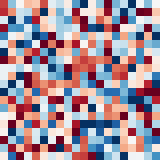
\includegraphics[width=0.4cm]{A}};
  \node[inner sep=0pt] at (0.24,0) {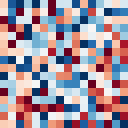
\includegraphics[width=0.4cm]{B}};
\end{scope}
\padlock{4.82}{1.98}
\chip[1.25]{1.75}{\sy}
\shield[0.95]{1.75}{1.6}{teeC}
\foreach \a/\b in {16.03/15.5,13.36/12.83,10.69/10.16,8.02/7.08}
  \draw[fo] (\a,\sy) -- (\b,\sy);
\draw[fo] (5.74,\sy) -- (4.9,\sy);
\draw[fo] (2.3,\sy) -- (3.7,\sy);
% deployment into the device
\draw[fo] (6.41,2.29) -- (6.41,3.94);
\draw[fo] (4.3,2.0) -- (4.3,6.13);
% prediction back to client (bridged over setup arrows)
\draw[f,bridge] (17.075,3.0) -- (17.075,2.8) -- (0.975,2.8) -- (0.975,3.08);
\node[n] at (11.0,2.8) {6};
\draw[f] (15.42,\ty) -- node[pos=0.5,n,above=1.5pt]{5} (16.45,\ty);
\end{tikzpicture}
\end{document}
